%+=+=+=+=+=+=+=+=+=+=+=+=+=+=+=+=+=+=+=+=+=+=+=+=+=+=+=+=+=+=+=+=+=+=+=+= PART
%+=+=+=+=+=+=+=+=+=+=+=+=+=+=+=+=+=+=+=+=+=+=+=+=+=+=+=+=+=+=+=+=+=+=+=+= PART
%+=+=+=+=+=+=+=+=+=+=+=+=+=+=+=+=+=+=+=+=+=+=+=+=+=+=+=+=+=+=+=+=+=+=+=+= PART
%+=+=+=+=+=+=+=+=+=+=+=+=+=+=+=+=+=+=+=+=+=+=+=+=+=+=+=+=+=+=+=+=+=+=+=+= PART
%+=+=+=+=+=+=+=+=+=+=+=+=+=+=+=+=+=+=+=+=+=+=+=+=+=+=+=+=+=+=+=+=+=+=+=+= PART
\newpage
\phantomsection\addcontentsline{toc}{section}{D\&D VOLUME II -- MONSTRES \& TRESORS}\begin{center}
{\Huge \ODDtitlefont{DONJONS \& DRAGONS}}{\normalsize \textsuperscript{\sffamily\textregistered}}

\vspace{1.8cm}

{\Large \textbf{Volume II}}

\vspace{1.3cm}

{\Huge \ODDtitlebisfont{MONSTRES \&}}

\vspace{0.3cm}

{\Huge \ODDtitlebisfont{TRESORS}}

\vspace{4cm}

{\large PAR

\vspace{0.1cm}

GARY GYGAX \& DAVE ARNESON}
\end{center}

\newpage

%======================Blank page
\phantom{-}
\newpage

%==========================================================================SECTION
\newpage
\phantomsection\section*{Monstres \& Trésors}
\addcontentsline{toc}{section}{Monstres \& Trésors}

\begin{center}
\textbf{[SELECTION]}
\end{center}

%----------------------------------------------------- SUB SECTION
\phantomsection\subsection*{\uline{DESCRIPTION DES MONSTRES :}}
\addcontentsline{toc}{subsection}{DESCRIPTION DES MONSTRES}

\pdfbookmark[3]{Nécrophage}{dd2-monstre-necrophage}\phantomsection\label{monstre-necrophage}\textbf{NECROPHAGE} : les nécrophages sont des créatures mauvaises qui drainent les niveaux d'énergie hors du corps de l'adversaire quand ils touchent en mêlée, un niveau par toucher. Ainsi, un toucher cause à la fois le dé de dommages et l'énergie correspondante pour se battre, ce qui signifie qu'un guerrier du neuvième niveau tomberait au huitième niveau. Les nécrophages ne peuvent pas être affectés par des armes de jet normales, mais les arcs aux flèches à pointe d'argent leur causeront des dommages normaux, et les flèches magiques leur causeront le double de dommages. Les armes magiques leur infligeront leurs dommages complets, et pour celles ayant un bonus spécial, ajouter le bonus aux dommages. Les humanoïdes tués par des nécrophages deviennent des nécrophages. Un opposant qui est complètement drainé de son énergie vitale par un nécrophage devient un nécrophage.

\bigskip

\pdfbookmark[3]{Rokh}{dd2-monstre-rokh}\phantomsection\label{monstre-rokh}\textbf{ROKHS} : ce terme a été utilisé pour désigner une catégorie de grands et fiers oiseaux ; le Rokh de la mythologie harcèle les éléphants ! Ainsi, les données fournies pour les Rokhs sont relatives aux petites variétés, et celles pour les plus grands des Rokhs devraient être doublées voire triplées. Tous les Rokhs font leur nid haut dans les plus inaccessibles des montagnes, et si une rencontre se produit alors que le Rokh est dans sa tanière, ce qui est en fait leur nid, il y a 50 \% de chances qu'il y ait entre 1--6 jeunes (œufs, poussins, ou oisillons). Les jeunes Rokhs peuvent être domestiqués et dressés pour servir de procréateurs. Les adultes sont toujours hostiles s'il y a des jeunes dans le nid. Sinon, ils seront positivement hostiles au Chaos et à la Neutralité, ignorant (80\%) ou étant amicaux (20\%) envers les personnages Bons qui ne tentent pas de s'approcher trop près.

%----------------------------------------------------- SUB SECTION
\phantomsection\subsection*{\uline{EXPLICATIONS DES OBJETS MAGIQUES :}}
\addcontentsline{toc}{subsection}{EXPLICATIONS DES OBJETS MAGIQUES}

%- - - - - - - - - - - - - - - - - - - - - - - - - - - SUB SUB SECTION
\phantomsection\subsubsection*{\uline{EPEES :}}
\addcontentsline{toc}{subsubsection}{EPEES}
\label{objet-epees}
{\parindent0pt

Parmi les armes magiques, seules les épées possèdent certains attributs humains (et surhumains) ; les épées ont un \myunderline{Alignement} (Loyal, Neutre ou Chaotique), un facteur d'\myunderline{Intelligence}, et un score d'\myunderline{Egoïsme} (ainsi qu'une détermination optionnelle de leur \myunderline{origine/objectif}). Ces déterminations sont faites de la manière suivante :

\bigskip

\pdfbookmark[4]{Alignement}{epees-align}\textbf{Alignement} : lancez un dé de pourcentage pour déterminer l'Alignement.

\bigskip

{\parindent2.5cm
\begin{tabular}{p{2.5cm}l}
01--65  & L'épée est Loyale \\
66--90  & L'épée est Neutre \\
91--00  & L'épée est Chaotique \\
\end{tabular}}

\bigskip

Notez que les pourcentages ci-dessus sont inversés pour l'épée ayant la capacité de drainer un niveau d'énergie vitale (83 sur la Table des Epées\footnote{Référence à la table des épées page 23 du livret original. Voir page \pageref{monstre-necrophage} pour la mécanique de drainage d'énergie (NdT).}). Si l'épée est Chaotique, elle affecte les créatures notées entre parenthèses (clercs, chevaux ailés, hippogriffes, rockhs, ents) au lieu de ceux indiqués en premier\footnote{Voir la table des épées.} (trolls et morts-vivants).

\bigskip

Si un personnage se saisit d'une épée qui n'est pas du même Alignement que lui-même, il subit les dommages suivants :

\bigskip

{\parindent2cm Loi -- Chaos : 2 Dés (2--12 points)

Neutralité - Loi/Chaos : 1 Dé (1--6 Points)}

\bigskip

Si on ordonne à un PNJ de prendre une épée, les dommages ne seront que de la moitié de ceux indiqués ci-dessus, car la personne n'agit pas de manière libre. De plus, l'épée pourrait libérer celui qui l'a prise d'un sortilège, le faire changer d'Alignement, ou alors lui faire gagner des pouvoirs, ce qui les enlèverait au précédent maître de l'épée.

\bigskip

De plus, si l‘Intelligence/Egoïsme de l'épée (voir ci-dessous) est supérieur de 6 points ou plus à celle du personnage qui l'a prise, l'épée contrôlera la personne, le faisant même prendre l'Alignement de l'épée, et agir en conséquence. Cela pourrait vouloir dire qu'un mercenaire d'un PJ Loyal à qui on ordonnerait de prendre une épée Neutre, et qui se ferait dominer par l'épée, mentirait délibérément à propos de ses pouvoirs ; si l'épée était Chaotique, il attaquerait.

\bigskip

Après avoir déterminé l'Alignement, il faut définir l'Intelligence de l'épée.

\bigskip

\pdfbookmark[4]{Intelligence}{epees-int}\myunderline{\textbf{Intelligence}} : l'Intelligence conditionne deux facteurs : les pouvoirs mentaux et la capacité à communiquer. Tous deux sont déterminés par un seul jet de dé.

\bigskip

\begin{tabular}{c l c}
\textbf{Intelligence}               &                                         & \textbf{Capacité de} \\
\textbf{\myunderline{(Jet de dé)}}  & \myunderline{\textbf{Pouvoirs mentaux}} & \myunderline{\textbf{communication}} \\
1--6    & Aucun                                         & Aucune* \\
7       & Un Pouvoir primaire                           & Empathie \\
8       & Deux Pouvoirs primaires                       & Empathie \\
9       & Trois Pouvoirs primaires                      & Empathie \\
10      & 3 Pouvoirs primaires et l'usage de langues**  & Parole \\
11      & Comme 10 plus Lecture de la Magie             & Parole \\
12      & Comme 11 plus une Capacité Extraordinaire     & Télépathie \\
\end{tabular}

\medskip

\begin{tabular}{rp{15.4cm}}
\multicolumn{1}{r}{*} & Même incapable de communiquer, l'épée confère au porteur ses pouvoirs, mais ceux-ci devront être découverts par l'utilisateur. \\
\multicolumn{1}{r}{**} & Le nombre de langues parlées \myunderline{en plus de la langue d'alignement de l'épée} est déterminé par un jet de dé. \\
\end{tabular}

\bigskip

\pdfbookmark[4]{Pouvoirs primaires}{epees-pouv}\begin{tabular}[t]{ll}

\begin{tabular}[t]{lp{7cm}}
\multicolumn{2}{l}{\myunderline{\textbf{Pouvoirs primaires}}} \\
\textbf{\myunderline{Jet de dés}} & \myunderline{\textbf{Pouvoir}} \\
01--15 & Remarquer des parois \& salles coulissantes \\
16--30 & Détecter des passages inclinés \\
31--40 & Localiser les portes secrètes \\
41--50 & Détecter les pièges \\
51--60 & Voir les objets invisibles \\
61--70 & Détecter le mal et/ou l'or \\
71--80 & Détecter la nourriture et son type \\
81--90 & Détecter la magie \\
91--95 & Détecter les bijoux (nombre et taille) \\
96--99 & Faire deux jets en ignorant les scores au dessus de 95 excepté 00 \\
\hspace{0.4cm}00 & Faire un jet sur la table des Capacités extraordinaires au lieu de celle-ci \\
\end{tabular}

\begin{tabular}[t]{lp{3cm}}
\multicolumn{2}{l}{\myunderline{\textbf{Langues parlées}}} \\
\textbf{\myunderline{Jet de dés}} & \myunderline{\textbf{Nb. langues}} \\
01--50 & Un \\
51--70 & Deux \\
71--85 & Trois \\
86--90 & Quatre \\
90--99 & Cinq \\
\hspace{0.4cm}00 & Faire deux jets en ignorant 00 s'il est tiré \\
\end{tabular}
\end{tabular}

\begin{center}
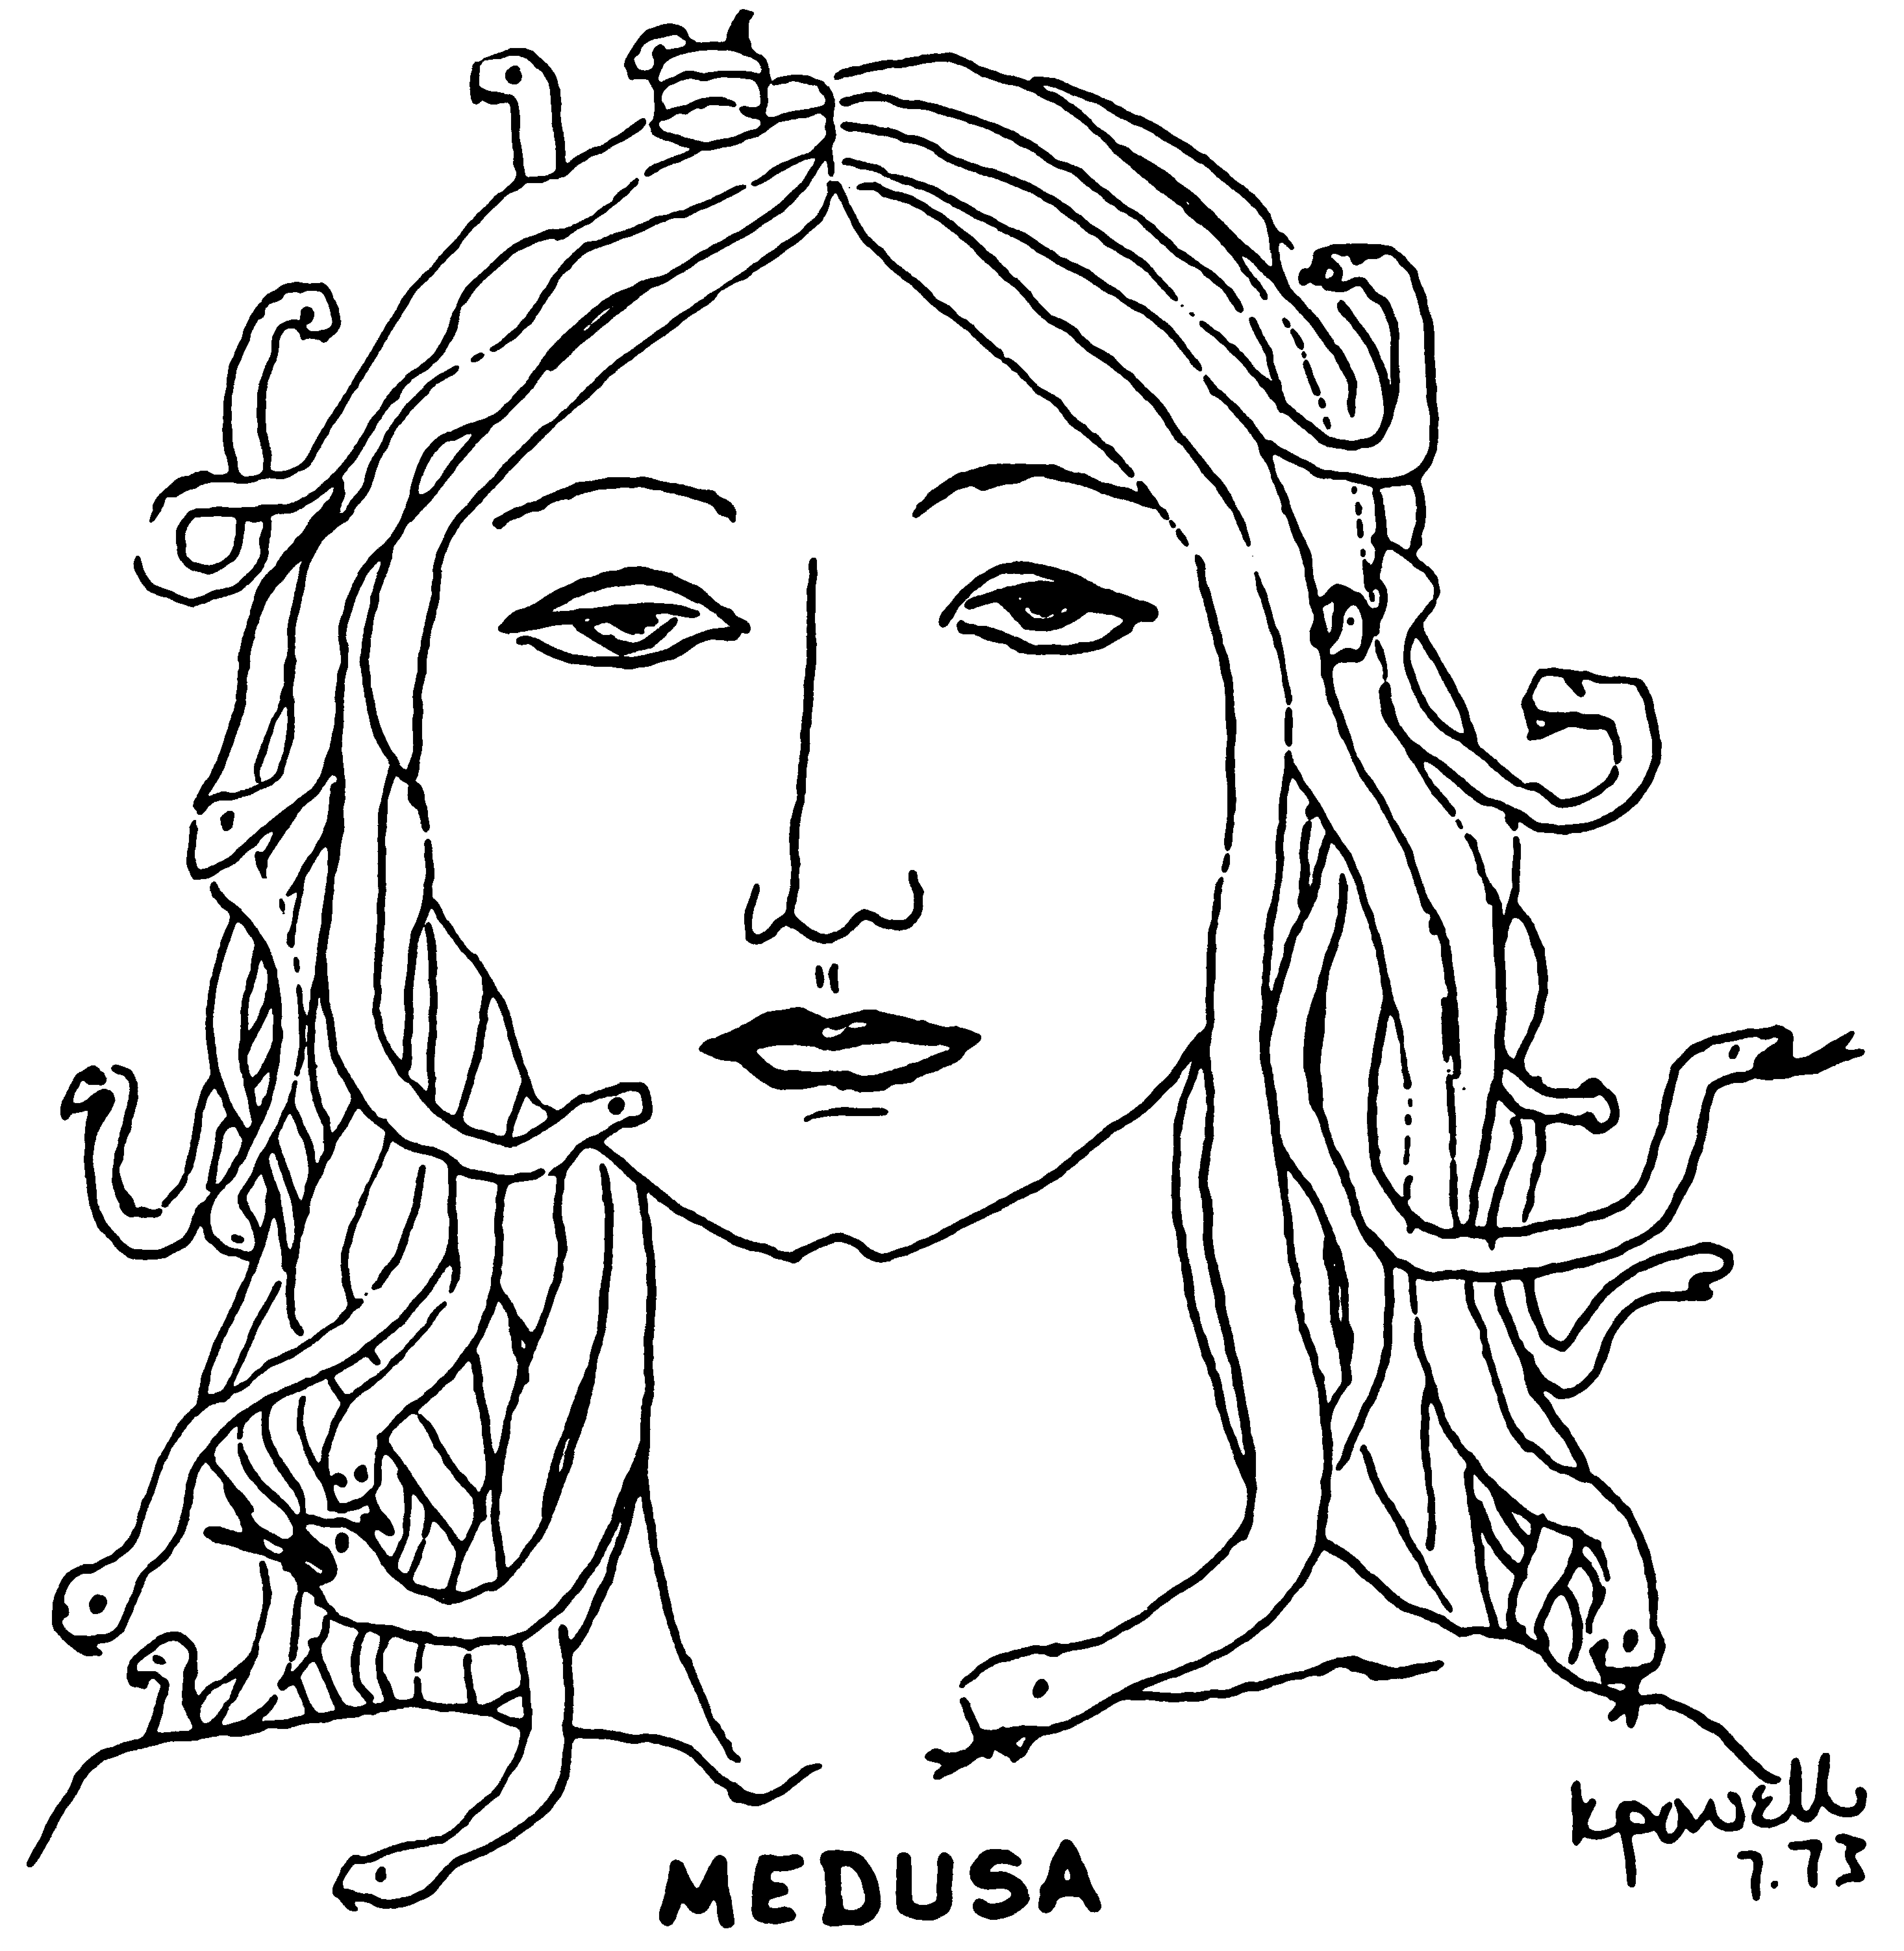
\includegraphics[scale=0.042]{./images/medusa.jpg}
\end{center}

\pdfbookmark[4]{Capacités extraordinaires}{epees-extra}\begin{tabular}[t]{p{3cm}p{12cm}}
\multicolumn{2}{l}{\myunderline{\textbf{Table des Capacités Extraordinaires}}} \\
\textbf{\myunderline{Jet de dé}} & \myunderline{\textbf{Capacité}} \\
01--10 & Clairaudience \\
11--20 & Clairvoyance \\
21--30 & Perception extrasensorielle \\
31--40 & Télépathie \\
41--50 & Télékinésie \\
51--59 & Téléportation \\
60--68 & Vision rayons X \\
69--77 & Génération d'illusions \\
78--82 & Lévitation \\
83--87 & Voler \\
88--92 & Soins (1 point/6 tours ou 6 points/jour) \\
93--97 & 1--4 fois la force normale pendant 1--10 tours, peut être employé une fois par jour \\
98-99 & Refaire deux jets en ignorant les jets au-dessus de 97 \\
\hspace{0.4cm}00 & Refaire trois jets en ignorant les jets au-dessus de 97 \\
\end{tabular}

\medskip

Tous les Pouvoirs primaires et Capacités extraordinaires sont transmis à l'utilisateur de l'épée. Si vous tirez la même capacité deux fois , cela signifie que la capacité est doublée en termes de force, de portée, de précision, etc.

\bigskip

\pdfbookmark[4]{Egoïsme}{epees-ego}\myunderline{\textbf{Egoïsme}} : seules les épées avec une Intelligence de 7 ou plus ont un score d'Egoïsme. L'Egoïsme est compris dans l'intervalle 1--12, plus le nombre est grand et plus grand est l'Egoïsme de l'épée. L'Egoïsme de l'épée peut lui faire faire les choses suivantes :

\begin{enumerate}
\item Obliger l'utilisateur à se défaire de meilleures armes,
\item Mettre l'utilisateur dans des situations très dangereuses afin d'exalter son rôle dans le combat,
\item Se laisser capturer par un personnage ou une créature de niveau plus élevé qui est plus proche de l'esprit de l'épée,
\item Se laisser capturer par un personnage ou une créature de niveau plus faible dans le but d'exercer un plus grand contrôle sur son utilisateur, et
\item Exiger qu'une partie des trésors conquis lui soit consacré, sous la forme de meilleurs fourreaux, d'incrustations de joyaux, ou de dispositifs magiques pour la garder quand elle n'est pas utilisée.
\end{enumerate}

A chaque moment où une situation se présente durant laquelle une des possibilités listées ci-dessus existe, l'Egoïsme de l'épée intervient. Ce dernier influencera toujours sa relation à l'utilisateur, bien que de vrais rapports puissent voir le jour si l'alignement et les buts du personnage/utilisateur coïncident avec l'\myunderline{origine/objectif} de l'épée. La détermination de chaque facteur est décrite ci-après:

\pdfbookmark[4]{Situations clef}{epees-situ}\begin{center}
\begin{minipage}{0.8\linewidth}
\textbf{Influence de l'Egoïsme dans des Situations Clef} : l'arbitre additionne l'Intelligence et l'Egoïsme de l'épée (facteurs entre 8 et 24) et ajoute 1 pour chaque Capacité Extraordinaire (entre 1--4 si applicable). Le total (8--28) est comparé au total de l'Intelligence et de la Force du personnage (6--36) modifié par une variable basée sur l'état physique de l'utilisateur. Si le personnage est frais et relativement exempt de dommages (moins de 10\% de dommages), il faut \myunderline{ajouter} 1--6 points à son total (de 7--42 est alors possible). S'il est mentalement ou physiquement fatigué, ou s'il a subi des dommages compris entre 10\% et 50\%, il faut \myunderline{déduire} 1--4 points de son total (de 2--35 est alors possible). Si les dommages subis dépassent les 50\%, ou le personnage a été sous le coup d'une tension mentale sévère venant d'une forme de magie, il faut \myunderline{déduire} 2--8 points (de 0--34 est alors possible).

\bigskip

{\parindent0.5cm \begin{tabular}{lcl}
\textbf{\myunderline{Différence}} && \myunderline{\textbf{Résultat}} \\
6 ou plus   && Le plus haut score l'emporte \\
2--5        && 75\% de chances que le plus haut score l'emporte \\
0--1        && 50\% de chances pour chacun \\
\end{tabular}}

\bigskip

\textbf{L'Egoïsme dans les relations au long cours avec l'utilisateur} : cette détermination est assez simple, car elle est basée sur la comparaison du score d'Egoïsme de l'épée (1--12) avec le niveau du guerrier l'utilisant. Consultez la table des \myunderline{Situations Clef} ci-dessus. Si l'une des parties a une différence positive de 6 ou plus, celle-ci l'emportera toujours et plus aucun test (incluant les Situations Clef) ne sera nécessaire. Une différence positive de 2--5 indiquera que celle ayant le plus haut score l'emporte généralement, et les tests ne devront être effectués que dans les Situations Clef. Une différence de 0--1 indique un combat continu entre l'épée et son utilisateur, et durant les situations stressantes, les deux devraient être testés afin de déterminer qui l'emporte.

\end{minipage}
\end{center}

\pdfbookmark[4]{Origine/objectif}{epees-origine}\myunderline{\textbf{Origine/Objectif}} : naturellement, l'origine de chaque épée est la Loi, la Neutralité ou le Chaos, mais certaines de ces armes sont forgées par des forces plus puissantes pour un objectif particulier. Pour déterminer si une épée possède un tel objectif, faire un jet de pourcentage et un jet de 91 ou plus indique que l'épée possède une mission spéciale. Les épées avec des objectifs spéciaux voient automatiquement leur score l'Intelligence et d'Egoïsme poussés au maximum et elles gagnent une capacité additionnelle :

\bigskip

{\parindent1cm \textbf{Loi}: la capacité de paralyser les opposants chaotiques

\textbf{Neutralité} : ajoute +1 à tous les jets de sauvegarde

\textbf{Chaos} : la capacité de désintégrer les opposants loyaux}

\bigskip

La capacité spéciale ne sera applicable que pour ceux que l'épée a été chargée de détruire, ou ceux qui les servent.

\myunderline{\textbf{Objectifs}}:

\medskip

{\parindent1.5cm\begin{tabular}{p{4.6cm}p{4.6cm}p{4.6cm}}
Tuer les magiciens & Tuer les guerriers & Vaincre la Loi \\
Tuer les clercs & Tuer les monstres & Vaincre le Chaos \\
\end{tabular}}

\bigskip

Ainsi, une épée au service de la Loi ayant pour but de tuer les magiciens (chaotiques) les paralysera ainsi que leurs sbires, mais elle n'utilisera pas ses pouvoirs de paralysie contre un géant errant. Néanmoins, les épées ayant un objectif large utiliseraient leurs pouvoirs pour vaincre tous les opposants de nature Loyale ou Chaotique. Les épées ayant un objectif spécial de Neutralité agiront contre la Loi et le Chaos de la même manière. Les épées ayant un objectif spécial chercheront toujours à l'accomplir, et chaque tentative de leurs utilisateurs de s'y opposer se soldera immédiatement par un test d'influence.

\bigskip

\pdfbookmark[4]{Bonus aux dommages}{epees-dom}\myunderline{\textbf{EPEES, BONUS AUX DOMMAGES}} : Les épées reçoivent toutes des bonus pour ce qui est de la probabilité de toucher un opposant, mais certaines d'entre elles reçoivent aussi un bonus aux dommages quand elles touchent. Ces épées sont celles qui ont un +2 ou +3 contre certaines créatures, mais pas celles qui ont un bonus général de +2 ou +3.



%- - - - - - - - - - - - - - - - - - - - - - - - - - - SUB SUB SECTION
\phantomsection\subsubsection*{DIVERS OBJETS MAGIQUES :}
\addcontentsline{toc}{subsubsection}{DIVERS OBJETS MAGIQUES}

\pdfbookmark[4]{Boules de cristal}{dd1-objet-boules}\phantomsection\label{objet-boule-cristal}\textbf{Boules de cristal} : généralement, l'utilisation réussie de ces objets est mise à mal par les grandes distances, quand le sujet n'est pas connu exactement, quand des sorts sont utilisés pour empêcher cette utilisation, quand du plomb s'interpose entre le magicien et le sujet, etc. Seulement trois tentatives par jour peuvent être faites dans les circonstances mentionnées ci-dessus sans rendre fou le magicien. Une utilisation longue de la boule de cristal demande au magicien de se reposer et de récupérer le jour suivant. Les sorts ne peuvent pas être lancés au travers d'une boule de cristal, mais l'opérateur peut, par exemple, lancer un sort d'infravision sur lui-même, puis regarder dans l'objet et voir dans les ténèbres.

\bigskip

\pdfbookmark[4]{Médaillons de perception extrasensorielle}{dd1-objet-medaillon-esp}\phantomsection\label{objet-medaillon-esp}\textbf{Médaillons de perception extrasensorielle} : ces objets sont utilisables par toutes les classes de personnages, même les Nains, mais l'objet dysfonctionne si l'on fait 6, donc quand il est utilisé, jeter un dé à six faces pour vérifier.

\bigskip

\pdfbookmark[4]{Amulette de captation}{dd1-objet-amulette-captation}\phantomsection\label{objet-amulette-captation}\textbf{Amulette de captation} : fonctionne avec une boule de cristal ou l'utilisation du sort Perception extrasensorielle\footnote{Voir page \pageref{sort-esp} (NdT).}. Cet objet donne la localisation, la vision, ou les pensées récupérées par la boule de cristal ou l'utilisation du sort. Il fonctionne en continu.

\bigskip

\pdfbookmark[4]{Heaume de télépathie}{dd1-objet-heaume-telepathie}\phantomsection\label{objet-heaume-telepathie}\textbf{Heaume de télépathie} : l'objet permet au porteur de lire les pensées de toute créature dans un rayon de 3m. Si son Intelligence est plus grande que la créature humaine ou humanoïde dans la portée du heaume, le porteur peut tenter de contrôler leur esprit avec des suggestions implantées de manière télépathique. De telles suggestions auront un effet de +2 dans leur probabilité d'être suivies (voir Vol. III pour les actions aléatoires des monstres\footnote{Voir page \pageref{dd3-actions-monstres} (NdT).}). Pour les personnages du jeu, faites un jet de pourcentage en ajoutant 10\% au porteur du heaume, et si le personnage échoue à battre ce score, il suivra la suggestion. (L'arbitre doit utiliser son jugement dans ce cas, car une suggestion de se suicider ne devrait pas avoir de chances d'être suivie par un événement.) Traiter comme un heaume non protégeant si le casque est porté en mêlée.

}% parindent


